\documentclass[10pt,conference,compsocconf]{IEEEtran}

\usepackage{hyperref}
\usepackage{graphicx}	% For figure environment
\usepackage{todonotes}

\long\def\/*#1*/{} % For long commentaries (ex: \/* my multiple-line comment */)

\begin{document}
\title{Higgs Boson: a Machine Learning Challenge}

\author{Timothée Duran, Marijn van der Meer, Bradley Mathez}

\maketitle
%%%%%%%%%%%%%%%%%%%%%%%%%%%%%%%%%%%%%%%%%%%%%%%%%%%%%%%%%%%%%%%%%%%%%%%%%%%%%%%%%%%%%%%%%%
%%% START DOCUMENT %%%%%%%%%%%%%%%%%%%%%%%%%%%%%%%%%%%%%%%%%%%%%%%%%%%%%%%%%%%%%%%%%%%%%%%
%%%%%%%%%%%%%%%%%%%%%%%%%%%%%%%%%%%%%%%%%%%%%%%%%%%%%%%%%%%%%%%%%%%%%%%%%%%%%%%%%%%%%%%%%%
\begin{abstract}
    \/* Below is the real text. I just kept the original text in comment.
    The goal of the written report is to show what you did and that you understand what you are doing. This does
    not mean that you need to explain everything that was shown in class. You can assume that the reader knows
    what cross-validation or gradient descent are. However, the reader should be able to reproduce your work, your results and understand why you made particular choices. Your choice of method need to be well motivated and you need to show evidence that your work has an elect.
    The simplest way to do so is to start with a simple model as a baseline, evaluate it, and a way to improve it, evaluate again and repeat. Explain the process that leads to your various improvements, evaluate the results carefully and present evidence using plots and tables.
    Cross validate
    Do not rely solely on the Kaggle/AICrowd submission system to get an error estimate. You need cross-validation to get an idea of the variance of your model.
    Tune Hyper-Parameters
    When comparing two models, make sure you tuned the hyper-parameters for both models beforehand.
    Comparing un-tuned / ill-defined models is not meaningful.
    Explain your decisions
    Do not throw a list of 10 methods you tried without explanation. We are more interested in your decision
    process than in what you tried.
    */
    
    This report explain the attempts we made for our participation in the Higgs boson machine learning challenge. This was a part of the Machine Learning course taught at EPFL. The goal was to find out through the given data from CERN if there are Higgs boson in the observations. We built different models that we optimized. This paper presents our results. 
\end{abstract}
%%%%%%%%%%%%%%%%%%%%%%%%%%%%%%%%%%%%%%%%%%%%%%%%%%%%%%%%%%%%%%%%%%%%%%%%%%%%%%%%%%%%%%%%%%
\section{Introduction}\label{sec: introduction}
    The Higgs boson is an elementary particle discovered at CERN. The data of this project comes from the experiment that allows the discovery of this particle, the ATLAS experiment and the CMS experiment. The Higgs boson can \textit{decay} in many different processes. It means that the Higgs boson produces specific particles when it decays. The idea of this project is to find these new particles groups, in other words,  to find its decay signature.
%%%%%%%%%%%%%%%%%%%%%%%%%%%%%%%%%%%%%%%%%%%%%%%%%%%%%%%%%%%%%%%%%%%%%%%%%%%%%%%%%%%%%%%%%%
\section{Models and Methods}\label{sec: models_methods}
    Describe your idea and how it was implemented to solve
    the problem. Survey the related work, giving credit where credit is
    due.
    \subsection{Data exploration and pre-processing}\label{subsec:data_cleaning}
    \subsection{Model implementation}
        \subsubsection{Parameters tuning}
            To tune the parameters of our model we performed a \textit{randomized grid search}. The idea is to give a range of values to each parameter. Then we pick $k$ random combinations of parameter's value among their respective range. After that we evaluate the model using cross validation. At each iteration we ensure that the value combination has not been tested before. We keep the results to compare them at the end and output the parameters value combination that gave the minimum average loss. This solution is faster that grid search or manual testing. We used this method on the following parameters: \todo{Fill}
%%%%%%%%%%%%%%%%%%%%%%%%%%%%%%%%%%%%%%%%%%%%%%%%%%%%%%%%%%%%%%%%%%%%%%%%%%%%%%%%%%%%%%%%%%
\section{Results}\label{sec: results}
    Organize the results section based on the sequence of table and
    figures you include. Prepare the tables and figures as soon as all
    the data are analyzed and arrange them in the sequence that best
    presents your findings in a logical way. A good strategy is to note,
    on a draft of each table or figure, the one or two key results you
    want to address in the text portion of the results.
    Show evidence to support your claims made in the
    introduction.
%%%%%%%%%%%%%%%%%%%%%%%%%%%%%%%%%%%%%%%%%%%%%%%%%%%%%%%%%%%%%%%%%%%%%%%%%%%%%%%%%%%%%%%%%%
\section{Discussion}\label{sec: discussion}
    Discuss the strengths and weaknesses of your
    approach, based on the results. Point out the implications of your
    novel idea on the application concerned.
%%%%%%%%%%%%%%%%%%%%%%%%%%%%%%%%%%%%%%%%%%%%%%%%%%%%%%%%%%%%%%%%%%%%%%%%%%%%%%%%%%%%%%%%%%
\section{Summary}\label{sec: summary}
    Summarize your contributions in light of the new
    results.
    The aim of a scientific paper is to convey the idea or discovery of
    the researcher to the minds of the readers. The associated software
    package provides the relevant details, which are often only briefly
    explained in the paper, such that the research can be reproduced.
    To write good papers, identify your key idea, make your contributions
    explicit, and use examples and illustrations to describe the problems
    and solutions.
%%%%%%%%%%%%%%%%%%%%%%%%%%%%%%%%%%%%%%%%%%%%%%%%%%%%%%%%%%%%%%%%%%%%%%%%%%%%%%%%%%%%%%%%%%
\subsection{Figures and Tables}

\begin{figure}[tbp]
  \centering
  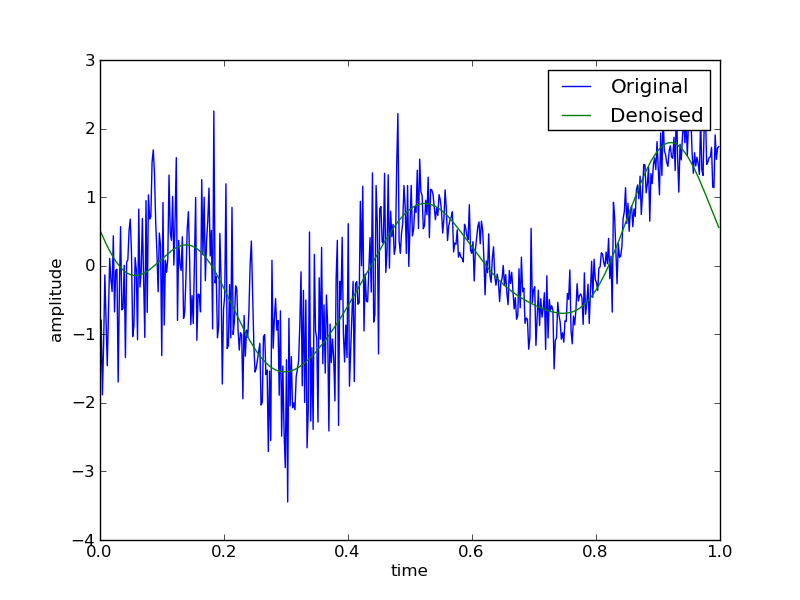
\includegraphics[width=\columnwidth]{denoised_signal_1d}
  \caption{Signal compression and denoising using the Fourier basis.}
  \vspace{-3mm}
  \label{fig:denoise-fourier}
\end{figure}
\begin{figure}[htbp]
  \centering
  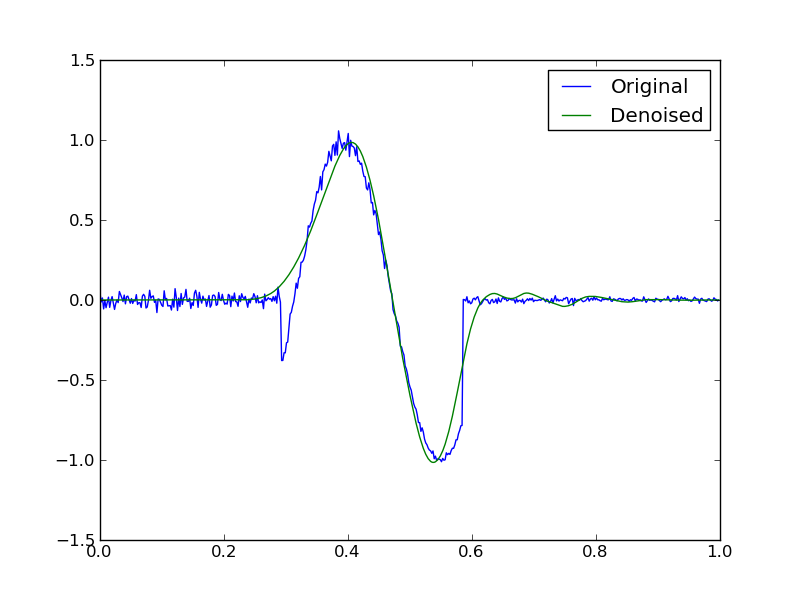
\includegraphics[width=\columnwidth]{local_wdenoised_1d}
  \vspace{-3mm}
  \caption{Signal compression and denoising using the Daubechies wavelet basis.}
  \label{fig:denoise-wavelet}
\end{figure}

Use examples and illustrations to clarify ideas and results. For
example, by comparing Figure~\ref{fig:denoise-fourier} and
Figure~\ref{fig:denoise-wavelet}, we can see the two different
situations where Fourier and wavelet basis perform well. 





\bibliographystyle{IEEEtran}
\bibliography{literature}

\end{document}
